% Options for packages loaded elsewhere
\PassOptionsToPackage{unicode}{hyperref}
\PassOptionsToPackage{hyphens}{url}
%
\documentclass[
]{book}
\usepackage{lmodern}
\usepackage{amssymb,amsmath}
\usepackage{ifxetex,ifluatex}
\ifnum 0\ifxetex 1\fi\ifluatex 1\fi=0 % if pdftex
  \usepackage[T1]{fontenc}
  \usepackage[utf8]{inputenc}
  \usepackage{textcomp} % provide euro and other symbols
\else % if luatex or xetex
  \usepackage{unicode-math}
  \defaultfontfeatures{Scale=MatchLowercase}
  \defaultfontfeatures[\rmfamily]{Ligatures=TeX,Scale=1}
\fi
% Use upquote if available, for straight quotes in verbatim environments
\IfFileExists{upquote.sty}{\usepackage{upquote}}{}
\IfFileExists{microtype.sty}{% use microtype if available
  \usepackage[]{microtype}
  \UseMicrotypeSet[protrusion]{basicmath} % disable protrusion for tt fonts
}{}
\makeatletter
\@ifundefined{KOMAClassName}{% if non-KOMA class
  \IfFileExists{parskip.sty}{%
    \usepackage{parskip}
  }{% else
    \setlength{\parindent}{0pt}
    \setlength{\parskip}{6pt plus 2pt minus 1pt}}
}{% if KOMA class
  \KOMAoptions{parskip=half}}
\makeatother
\usepackage{xcolor}
\IfFileExists{xurl.sty}{\usepackage{xurl}}{} % add URL line breaks if available
\IfFileExists{bookmark.sty}{\usepackage{bookmark}}{\usepackage{hyperref}}
\hypersetup{
  pdftitle={A Person-Centered Framework},
  pdfauthor={Various authors},
  hidelinks,
  pdfcreator={LaTeX via pandoc}}
\urlstyle{same} % disable monospaced font for URLs
\usepackage{longtable,booktabs}
% Correct order of tables after \paragraph or \subparagraph
\usepackage{etoolbox}
\makeatletter
\patchcmd\longtable{\par}{\if@noskipsec\mbox{}\fi\par}{}{}
\makeatother
% Allow footnotes in longtable head/foot
\IfFileExists{footnotehyper.sty}{\usepackage{footnotehyper}}{\usepackage{footnote}}
\makesavenoteenv{longtable}
\usepackage{graphicx,grffile}
\makeatletter
\def\maxwidth{\ifdim\Gin@nat@width>\linewidth\linewidth\else\Gin@nat@width\fi}
\def\maxheight{\ifdim\Gin@nat@height>\textheight\textheight\else\Gin@nat@height\fi}
\makeatother
% Scale images if necessary, so that they will not overflow the page
% margins by default, and it is still possible to overwrite the defaults
% using explicit options in \includegraphics[width, height, ...]{}
\setkeys{Gin}{width=\maxwidth,height=\maxheight,keepaspectratio}
% Set default figure placement to htbp
\makeatletter
\def\fps@figure{htbp}
\makeatother
\setlength{\emergencystretch}{3em} % prevent overfull lines
\providecommand{\tightlist}{%
  \setlength{\itemsep}{0pt}\setlength{\parskip}{0pt}}
\setcounter{secnumdepth}{5}
\usepackage{booktabs}
\usepackage[]{natbib}
\bibliographystyle{apalike}

\title{A Person-Centered Framework}
\author{Various authors}
\date{2020-05-20}

\begin{document}
\maketitle

{
\setcounter{tocdepth}{1}
\tableofcontents
}
\textbf{This document is currently a work in progress and is not intended for distribution outside of those collaborating on its development with the direction of MDHHS-BHDDA.}

\hypertarget{reason}{%
\chapter{Reason}\label{reason}}

This framework arises from a simple conviction: the intent of supports and services is to help each person flourish, to achieve a better life.

That belief is thankfully not a new one. It aligns with the person-centered planning policy\citep{pcp-policy} published by the Michigan Department of Health and Human Services' \emph{Behavioral Health and Developmental Disabilities Administration} (MDHHS-BHDDA), which begins by stating that:

\begin{quote}
\emph{The purpose of the community mental health system is to support adults and children\ldots{} to live successfully in their communities --- achieving community inclusion and participation, independence, and productivity {[}and to{]} to identify and achieve their personal goals.}
\end{quote}

The framework defined below is an attempt to apply these longstanding and fundamental values in a way that allows for consistent definitions, implementation, and evaluation.

Each person has the ability to choose a better future, to chart a course toward it and strive to reach it: person-centered planning provides a platform to enable this process. In order for services to effectively support a person in this process, they must be provided within the context of a person's goals. Orienting a broad and complex system to keep the person as its central focus requires a consistent, overarching framework. MDHHS-BHDDA is working to support this person-centered orientation with the following strategy:

\textbf{Goal:} To develop \protect\hyperlink{bok}{a common body of knowledge} for person-centered planning,
mapped to \protect\hyperlink{policy}{relevant policies} and \protect\hyperlink{research}{research},
which will inform a \protect\hyperlink{curriculum}{shared curriculum}
and \protect\hyperlink{measure}{measurement framework}
to support \protect\hyperlink{pcpdca}{improved quality of life} for each person.

\hypertarget{pcpdca}{%
\chapter{Person-Centered Planning (\ldots Doing, Checking, Acting)}\label{pcpdca}}

Person Centered Planning upholds the truth about healthcare; while healthcare continues to focus on treating groups and classes of diagnoses, change is ultimately driven by the individual person. This is the profound insight of \emph{person-centered planning} (PCP), which has long been the cornerstone of Michigan policy related to behavioral health services and supports.\footnote{See \citet{mi-mhc}.}

While putting forward specific definitions of person-centered planning and its parts will be a focus of \protect\hyperlink{bok}{later sections of this document}, it is worth noting at the outset that our goal is to adopt a broader scope for person-centered planning than is often seen in practice\footnote{Even though this broader definition does conform to existing policy and guidance}. This is because, despite the central position of PCP to policy regarding Medicaid supports and services in Michigan, its practice has often been relegated to the planning meeting itself and the preparation for that meeting: ensuring inclusion of family and friends, personal involvement, etc. While the act of developing a plan remains a cornerstone of the process, it is only one step needed to truly achieve one's goals.\footnote{Part of the focus on the meeting is due to the auditing focus on the plan document: an instance of \emph{what is measured, is addressed}. This should serve as an abiding reminder during the implementation of the framework defined here, that there are unintended consequences to measurement.}

In this document, the phrase \emph{person-centered planning} is used broadly, to encompass not only the initial planning process but also its implementation, monitoring, and refinement. The extension of this definition beyond the PCP meeting and document into a framework which directs all services and supports is already recognized within state policy\footnote{See \citet{pcp-policy}, p.~1}, which indicates that:

\begin{quote}
\emph{through PCP, a person is engaged in decision-making, problem solving, monitoring progress, and making needed adjustments to goals and supports and services provided in a timely manner.}
\end{quote}

The table below suggests how existing paradigms can be used to augment these policy requirements and be incorporated into our framework. Here we makes use of paradigms for \protect\hyperlink{qol_intro}{Quality of Life} (QoL), \protect\hyperlink{comb_intro}{behavior change} (\emph{Capability-Opportunity-Motivation-Behavior}, or COM-B), and \protect\hyperlink{pdca_intro}{continual improvement} (\emph{Plan-Do-Check-Act}, or PDCA):

\begin{table}

\caption{\label{tab:unnamed-chunk-3}Paradigms related to PCP}
\centering
\begin{tabular}[t]{l|l|l|l}
\hline
Paradigm & Tells us & Relates to & Answers\\
\hline
QoL & Why? & Vision for a better life & What areas of life do I want to focus on?\\
\hline
COM-B & What? & Turning vision into plan & How will I start to address my goal?\\
\hline
PDCA & How? & Making my plan work & How is the plan working? How to change?\\
\hline
\end{tabular}
\end{table}

\hypertarget{qol_intro}{%
\section{Vision for a Better Life}\label{qol_intro}}

Priorities and choices vary from person to person, yet many dimensions of what makes a good life are broadly agreed upon across people and cultures\footnote{For more detail, see the quality of life definitions \protect\hyperlink{qol_def}{in the measurement discussions} section.}: \emph{choice, relationships, access to needed resources, physical and emotional well-being}\ldots{} these are some of the dimensions which we collectively refer to as quality of life.

People usually seek services and supports because they see a gap between their current situation and a better life. Person-centered planning encourages a person to cast a vision for their lives and to identify gaps between their hopes and their current situation. In order to ensure a comprehensive approach, it is valuable to prompt consideration across all QoL domains in identifying goals.

\hypertarget{comb_intro}{%
\section{Turning Vision into Plan}\label{comb_intro}}

Once a person has set a vision for a better life and identified gaps between where they are and where they want to go, a map needs to be drawn. This map draws potential routes to connect a person from where they are to where they want to be.

The COM-B model for behavioral change, an acronym for \emph{Capability-Opportunity-Motivation-Behavior} provides a way to map out these routes. It helps to conceptualize the facilitators and barriers to changing one's life. Note that the goals addressed are not limited to ``challenging behaviors'' or related to medical issues (\emph{e.g.~weight loss, or quitting smoking}). The behavior addressed could be as simple as any broad goal related to quality of life.

Visualized in the graphic below:\footnote{Source of image: \citet{comb-pic}}

\begin{figure}
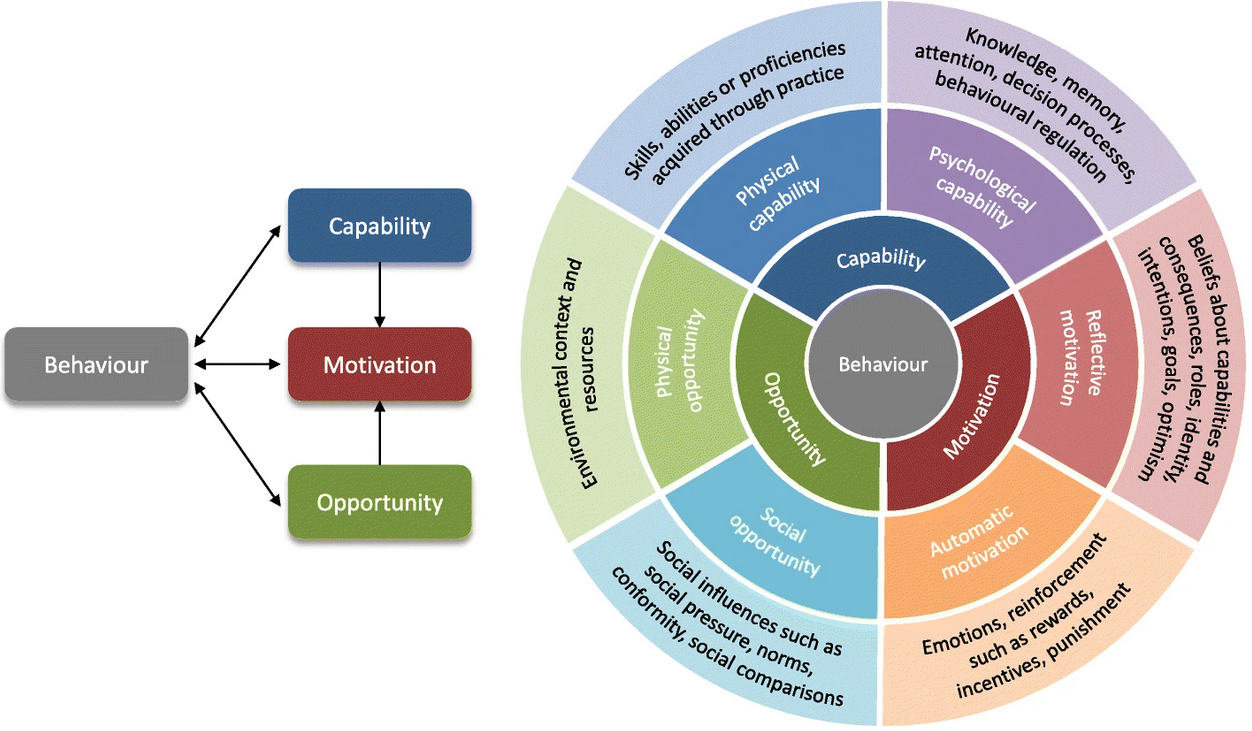
\includegraphics[width=31.3in]{_bookdown_files/img/com-b} \caption{The COM-B Model}\label{fig:unnamed-chunk-4}
\end{figure}

For instance, a person may have a goal to enrich the relationship with his/her parents. The person's \emph{capability} to enrich that relationship may be strained by previous trauma, difficulty communicating, or other challenges. Perhaps they would benefit from trauma-focused therapy or simply some coaching and modelling of how to engage in difficult conversations. If the person's parents live across town, but he/she does not have access to reliable transportation, then there is also the need to create \emph{opportunity} to reach that goal. This might entail gettig a bus pass, finding other transportation and additionally setting up access to phone calls or other communication platforms (e.g.~FaceTime or Skype). In this case, the person's motivation is already present. In some other cases, such as nutrition or smoking cessation, there is often an need for \emph{motivation}al assistance as well.

In the example above, one is thinking through \emph{Capacity}, \emph{Opportunity}, and \emph{Motivation} in order to generate ideas about how to achieve a prioritized goal. The ideas which are generated (e.g.~coaching on difficult conversations, getting a bus pass, etc.) are akin to what have typically been called \emph{objectives} in person-centered planning. These are the steps that a person wants to pursue in order meet a broader \emph{goal} to improve quality-of-life.

Note that objectives or supports identified above are not the only ones which could possibly get a person to their goal. It may actually be the case that writing hand-written notes would be more helpful in getting this particular person to establish a closer relationship with their parents. This is why a particular set of objectives should be viewed as a personal experiment in improving one's life. The objectives form a hypothesis, where one is saying that doing a set of activities will facilitate the achievement of a goal. There is no reason to think that a person's first hypothesis will be correct, or even that the hypotheses of loved ones or experts must be correct.

This is where iteration and the improvement cycle come in\ldots{}

\hypertarget{pdca_intro}{%
\section{Making My Plan Work}\label{pdca_intro}}

The \emph{Plan-Do-Check-Act} (PDCA) cycle is a simple model for implementing a change and checking to see if it is working.\footnote{While there are various other rubrics related to learning and improvement, PDCA has been selected here because of its use of `planning' language, its simplicity, and its familiarity among behavioral healthcare providers and funders.} The \emph{QoL} and \emph{COM-B} frameworks discussed above provide a way to identify goals and design individualized strategies to meet those goals: they fall into the \emph{Plan} phase of the PDCA cycle.

As the intent of supports and services is to improve personal quality of life, practitioners can view the PCP process as similar to the PDCA cycle, which involves many elements of the broader scope of PCP referred to above. Versions of the PDCA cycle have already been successfully incorporated into the supports and treatment planning process for people with varying conditions and needs, from intellectual and developmental disabilities, to mental illness, to physical health concerns.

If we want to understand whether a person's plan is supporting his/her goals, it is necessary to have a strategy to measure improvement in the person's desired areas of focus. Such measurement-based approaches have been gaining traction in their use across populations and been implemented in a manner which is valued by people receiving services.\footnote{\citet{shalock-changes} notes ``an increased emphasis on\ldots{} conducting outcome evaluation\ldots{} to assess the degree to which personal goals, positive changes, or benefits have been achieved'' in IDD planning.}

Framing the intent of supports and services as improving personal quality of life through planning creates a natural bridge to using well-tested quality improvement processes at the individual level. Rather than assuming that an objective will lead to the desired goal as it is initially written, this approach allows for trying out different approaches and revising them to find what works, in the spirit of continuous quality improevment.

\begin{figure}
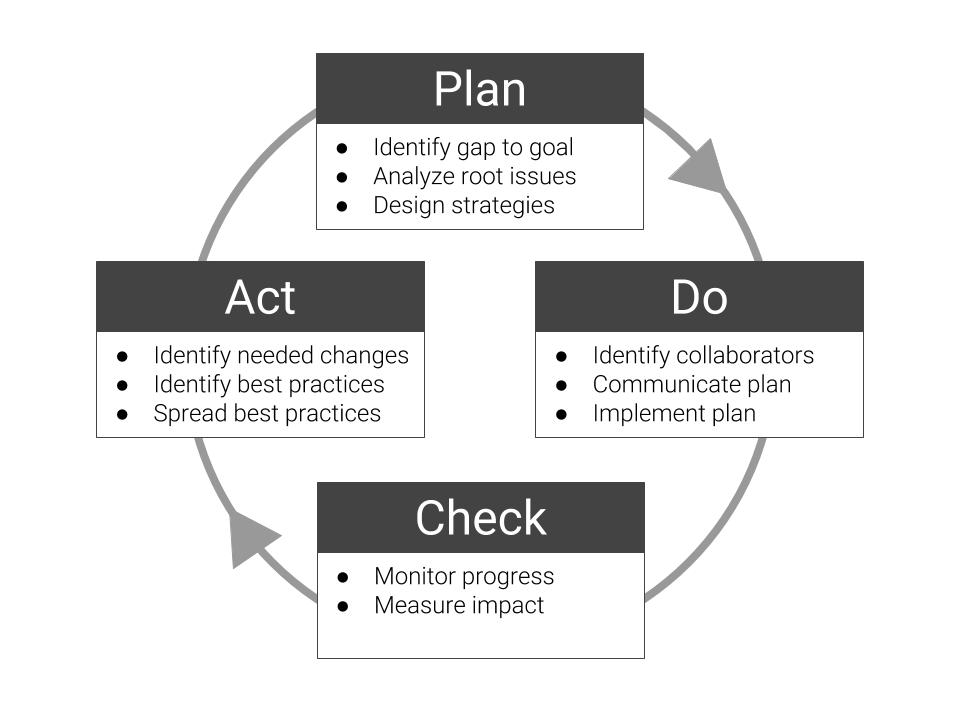
\includegraphics[width=24in]{_bookdown_files/img/pdca} \caption{PDCA cycle applied to PCP process}\label{fig:unnamed-chunk-5}
\end{figure}

The table below illustrates the relationship between the PDCA process and a fuller definition of the PCP process:

\begin{table}

\caption{\label{tab:unnamed-chunk-6}Alignment of PDCA and PCP}
\centering
\begin{tabular}[t]{l|l|l|l|l}
\hline
Factor & Plan & Do & Check & Act\\
\hline
*Questions* & What is your life like? & What are you working on? & Is life better? & What next?\\
\hline
 & What do you want to pursue? & How are supports provided? &  & How to improve approach?\\
\hline
 & What supports do you need? &  &  & \\
\hline
*Activities* & Identify QoL & Work on plan & Check QoL & Revise plan\\
\hline
 & Assess needs & Coordinate services & Reassess needs & (Repeat cycle)\\
\hline
 & Develop plan &  &  & \\
\hline
*Quality area* & Structure & Process & Outcome & (Re)structure\\
\hline
\end{tabular}
\end{table}

Note that, while the questions above can be tied to various data-points\footnote{See the \protect\hyperlink{measure}{section on measurement} for examples of how this might be accomplished.}, it is most important that they should be conversational: founded upon an ongoing process of personal striving for improvement.

\hypertarget{bok}{%
\chapter{A Common Body of Knowledge}\label{bok}}

As a foundation for this effort, MDHHS has begun to develop a shared repository of key terms and concepts, their definitions, and how they are related to one another. This common language has the following key features:

\begin{itemize}
\tightlist
\item
  Relates all terminology back to the person, who drives service delivery
\item
  Includes concepts related to the PCP process, as broadly defined above, as well as common attributes for understanding the person\footnote{Note that the body of knowledge is not intended to classify services and supports.}
\item
  Promotes consistency in implementation and training, and a platform for future development
\item
  Allows for change; the language can be extended as new concepts are identified.\footnote{This approach also requires that ideas claiming to be new must differentiate themselves from existing terms and concepts.}
\item
  Reduces confusion across various policies with inconsistent terminology and scope
\end{itemize}

\hypertarget{what-is-a-body-of-knowledge}{%
\section{What is a Body of Knowledge?}\label{what-is-a-body-of-knowledge}}

\begin{quote}
``If you wish to converse\ldots{} define your terms.''

--- Voltaire
\end{quote}

Person-centered thinking and planning should never become rote, and continue to be a part of a living dialogue. Dialogue and consistent implementation require a shared language.\footnote{According to Will Durant, this requirement is ``the heart and soul of {[}logic{]}, that every important term\ldots{} be subjected to strictest scrutiny and definition. It is difficult, and ruthlessly tests the mind; but once done it is half of any task.'' \citet{durant}}

Our purpose here is to identify and define concepts related to person-centered planning. This is done in a way which connects core concepts to both state and federal regulations. This collection of core concepts is intended to serve as an evolving, foundational outline for a body of knowledge; encompassing person-centered thinking, planning, implementation and monitoring.\footnote{Please note that the current work aims at an initial proof-of-concept, and not as a process ready for automation or scaling.}

\hypertarget{potential-uses}{%
\section{Potential Uses}\label{potential-uses}}

Potential uses of this body of knowledge include the following:

\begin{itemize}
\tightlist
\item
  \emph{Policy Search}: searching of existing policies in electronic format to identify requirements related to each core concept
\item
  \emph{Impact of Policy Changes}: identification of relevant new federal policy requirements to allow for clear understanding of which current policies are related and complicated by the new federal policy
\item
  \emph{Basis of Curriculum}: serving as the foundation of \protect\hyperlink{curriculum}{a standard curriculum} to train people receiving services, their families, direct-care team members, supports coordinators, case managers, clinicians, and others about the PCP process.
\item
  \emph{Monitoring Quality}: allowing for \protect\hyperlink{measure}{system-level monitoring of the quality of PCP practice}, through measurements and/or the use of a best practice review model.\footnote{This could be developed similar to the MI-FAST model, which has been used to review the fidelity to evidence-based practices.}
\item
  \emph{Promising Practices}: use of key terms for ongoing literature review and meta-analysis of PCP-related practices in the research literature, to build \protect\hyperlink{research}{a base of best practices and evidence for effectiveness}.
\end{itemize}

\hypertarget{identifying-core-concepts}{%
\section{Identifying Core Concepts}\label{identifying-core-concepts}}

\hypertarget{what-makes-a-concept-a-core-concept}{%
\subsection{What makes a concept a `core' concept?}\label{what-makes-a-concept-a-core-concept}}

In order to compile relevant policies and guidance related to person-centered planning, we selected and defined an initial set of core concepts related to person-centered planning. The `source of truth' for these concepts was state-level policy in Michigan, since this is the level at which shared dialogue and consistent implementation is sought.

The following methods were used to develop this initial set of core concepts:

\begin{itemize}
\tightlist
\item
  \textbf{Manual review and annotation} of documents which define person-centered planning in the Michigan Public Behavioral Health System. These include (a) the Person-Centered Planning Policy\footnote{\citet{pcp-policy}}, (b) the Self-Determination Policy and Practice Guideline\footnote{\citet{sd-policy}}, and (c) the Michigan Mental Health Code section 330.1712 Individualized written plan of services\footnote{\citet{mi-mhc}}.
\item
  \textbf{Identifying synonyms} For instance, the term \emph{person} was mapped to the similar terms \emph{person, personal, patient, individual, client, consumer, recipient, beneficiary}. This was done for all core concepts in order to identify their occurrence across multiple policies.
\item
  \textbf{Comprehensive annotation} for the policies referenced above, to assure that the most commonly used terms and phrases were included as core concepts.
\end{itemize}

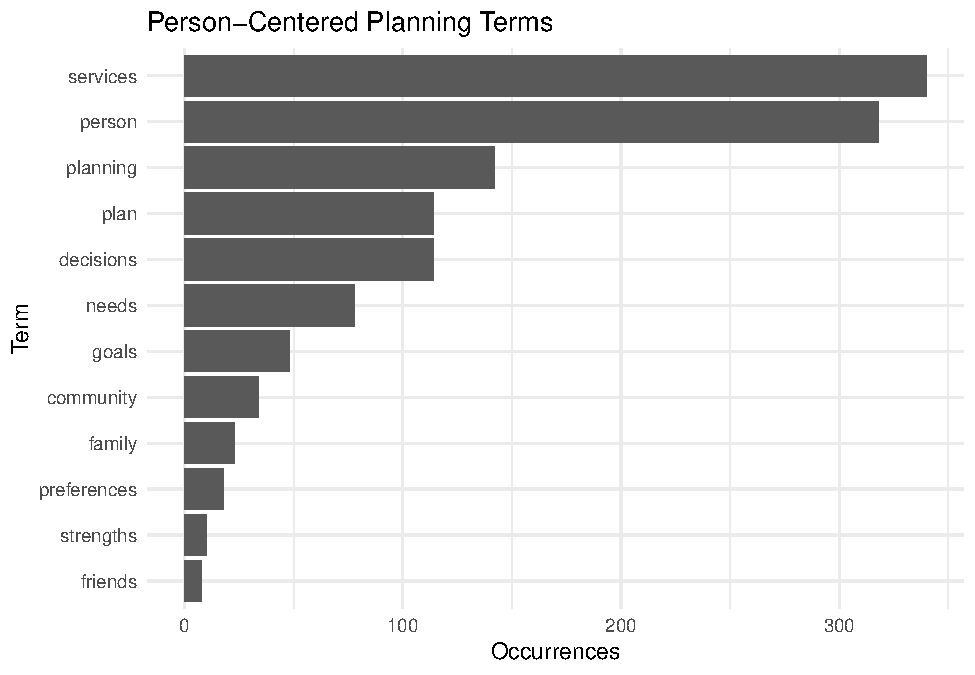
\includegraphics{person_centered_files/figure-latex/plot_concept-1.pdf}

\begin{itemize}
\tightlist
\item
  \textbf{Purposeful Word Choice.} We select a distinct, `master' term to refer to various synonyms across documents. The selection of terms is informed by a consistent set of principles.
\end{itemize}

\hypertarget{characteristics-of-a-person}{%
\subsection{Characteristics of a Person}\label{characteristics-of-a-person}}

To honor the person in the language used, and to do so simply, we define each person as having the following features:

\begin{itemize}
\tightlist
\item
  \textbf{description}: a set of characteristics specific to the person, defined by that person and those who know the person well.
\item
  \textbf{connections}: the people, places and things which make up the context of a person's life
\item
  \textbf{direction}: what the person intends for his/her life to become, by imagining a future and making choices to move toward it
\end{itemize}

Note that these are features of being human for all of us. The intent of this framework is to describe attributes of a person which are more broadly human, and not merely focused on illness or disability. While this framework is intended for implementation with Medicaid public behavioral health recipients, the approach outlined here should apply to any reader: from legislators to clinicians, from administrators and direct-care workers.

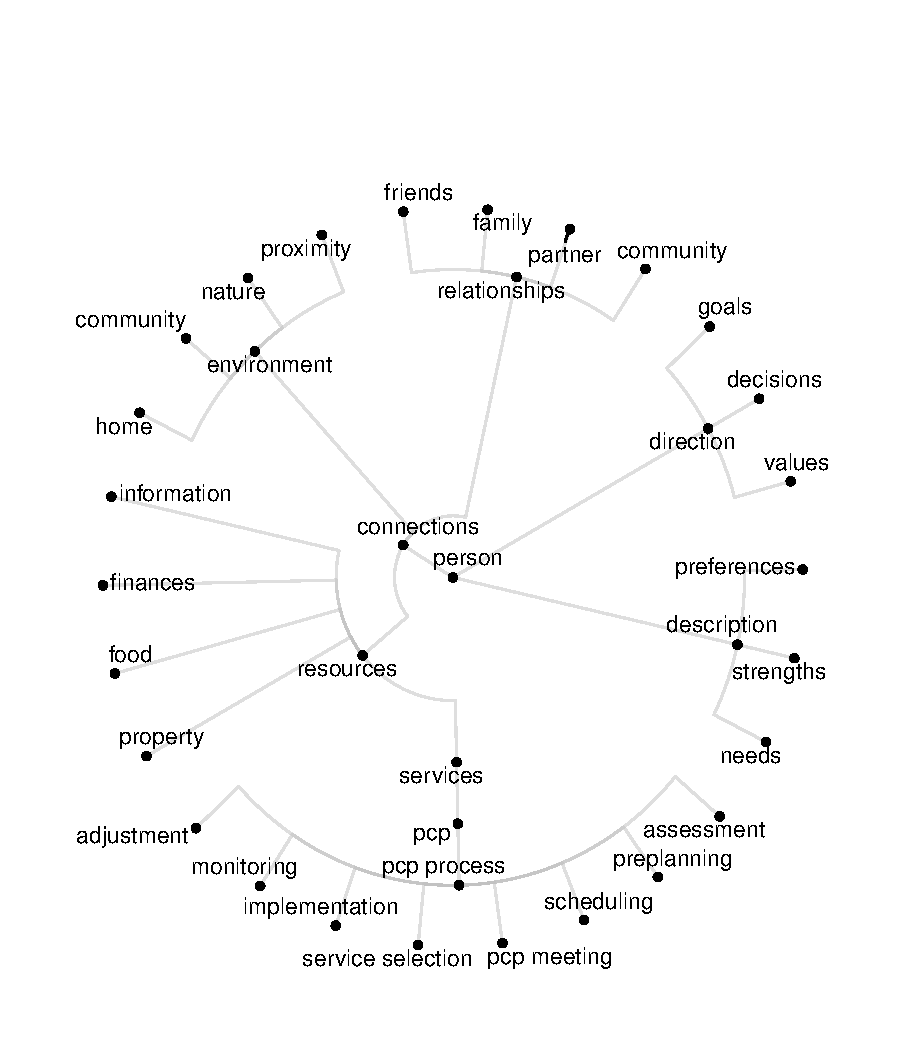
\includegraphics{person_centered_files/figure-latex/unnamed-chunk-8-1.pdf}

Each element of the person-centered planning framework is shown above. Each concept is defined by its relation with other concepts, as well as having a distinct definition, as shown below.

\hypertarget{define}{%
\section{Defining Core Concepts}\label{define}}

Defining core concepts and terms, using policy where possible.

\begin{table}

\caption{\label{tab:unnamed-chunk-9}Concept Definitions and Synonyms}
\centering
\begin{tabular}[t]{l|l|l}
\hline
Concept & Definition & Synonyms\\
\hline
description & Features which can be attributed to the person, as opposed to his/her connections, environment, etc. & attributes; characteristics\\
\hline
direction & The aspects of the person which allow him/her to imagine a future and to plan and work to achieve it & personal intent; aspiration\\
\hline
connections & The relationships which a person has to the people, places and things around them & circumstance;circumstances;opportunity\\
\hline
relationships & Natural relationships which the person has with other people.  Does not include economic relationships or interactions with "systems". & natural supports\\
\hline
environment & The physical context in which the individual lives; here referring to the non-human environment including shelter and the natural world. & location;setting;environment\\
\hline
\end{tabular}
\end{table}

\hypertarget{policy}{%
\chapter{Comprehensive Mapping to Policy}\label{policy}}

As with any important idea, person-centered planning has been discussed and debated for decades, leaving a vast body of policy, regulations, guidance, and explanations to sift through. While the basic idea of person-centered planning is simple and commonsense, practitioners are also required to adhere to complex existing policies. With this in mind, the body of knowledge is being developed:

\begin{itemize}
\tightlist
\item
  Based on a broad scope of relevant state and federal policies identified by MDHHS-BHDDA.
\item
  Using natural-language processing techniques to identify and refine core terminology from the text of the identified policies
\item
  In a manner that allows MDHHS-BHDDA to identify whether new federal policies would align with the current implementation of PCP
\end{itemize}

\hypertarget{identify-scope-of-policy}{%
\section{Identify Scope of Policy}\label{identify-scope-of-policy}}

In collaboration with policy experts at MDHHS-BHDDA, we identified this initial set of state and federal regulations:

\begin{table}

\caption{\label{tab:unnamed-chunk-10}Regulations included in PCP body of knowledge.}
\centering
\begin{tabular}[t]{l|l|l}
\hline
Source & Abbreviated Title & Regulation\\
\hline
MI-State & Self-D & Self-Determination Policy \& Practice ...\\
\hline
MI-State & PCP & Person-Centered Planning\\
\hline
MI-State & MHCode & Mental Health Code\\
\hline
MI-State & Mcaid-PM & Medicaid Provider Manual\\
\hline
MI-State & AFC-TA & Adult Foster Care Group Homes Technic...\\
\hline
MI-State & AFC-SC & Certification of Specialized Programs...\\
\hline
MI-State & AFC-Act & AFC Facility Licensing Act 218 of 1979\\
\hline
MI-State & AFC-12 & Licensing Rules for AFC Small Group H...\\
\hline
Federal & Parity & Medicaid and Children's Health Insura...\\
\hline
Federal & No-Wrong-Door & Agency Information Collection Activit...\\
\hline
Federal & MU-Medicaid & Medicare Program; Hospital Inpatient ...\\
\hline
Federal & MU-EHR & 2015 Edition Health Information Techn...\\
\hline
Federal & MH-BG & Mental Health Block Grants\\
\hline
Federal & MCMC-Rx & Medicare and Medicaid Programs; Polic...\\
\hline
Federal & Mcare-Adv & Agency Information Collection Activit...\\
\hline
Federal & Mcare-ACO-Waiver & Medicare Program; Medicare Shared Sav...\\
\hline
Federal & Mcare-ACO-Savings & Medicare Program; Medicare Shared Sav...\\
\hline
Federal & Mcaid-ManagedCare & Medicaid and Children's Health Insura...\\
\hline
Federal & LTC-Reform & Medicare and Medicaid Programs; Refor...\\
\hline
Federal & HCBS & Medicaid Program; State Plan Home and...\\
\hline
Federal & ELTSS & Medicaid and Children's Health Insura...\\
\hline
Federal & Discharge & Medicare Program; Hospital Inpatient ...\\
\hline
Federal & CCHBC & CCHBC Requirements\\
\hline
Federal & ACA-Market- & Patient Protection and Affordable Car...\\
\hline
Federal & ACA-Benefit & Patient Protection and Affordable Car...\\
\hline
\end{tabular}
\end{table}

This set of policies and regulations can be expanded as necessary.\footnote{For example, using the Federal Register API to \href{https://www.federalregister.gov/documents/search?conditions\%5Bagencies\%5D\%5B\%5D=centers-for-medicare-medicaid-services\&conditions\%5Bagencies\%5D\%5B\%5D=health-and-human-services-department\&conditions\%5Bagencies\%5D\%5B\%5D=substance-abuse-and-mental-health-services-administration\&conditions\%5Bterm\%5D=person-centered\&conditions\%5Btype\%5D\%5B\%5D=RULE\#}{search for policies} containing the phrase ``person-centered'' by relevant agencies.} Additional work will be needed to assure that the most current version of amended policies is used, as this approach is refined.

\hypertarget{find-occurrence-of-concepts-in-policy}{%
\section{Find Occurrence of Concepts in Policy}\label{find-occurrence-of-concepts-in-policy}}

The core concepts are derived from key policy documents, as defined in \protect\hyperlink{bok}{the previous section}, which allows for related terms to be flagged within other policy documents. One of the most challenging issues facing any attempt to give clear, consistent, and comprehensive guidance related to person-centered planning is the large, diverse, and continually evolving set of requirements and guidance.

The previous section outlined the process for deriving key concepts from state-level policies and guidelines. The next step is to identify these concepts when they occur within a much larger set of federal policies. This will allow for policy specialists to:

\begin{itemize}
\tightlist
\item
  suggest necessary refinements to the body of knowledge
\item
  identify relevant requirements which were previously unknown
\item
  identify potential discrepancies between policies which address a similar concept
\end{itemize}

To do this, this analysis maps policy words and phrases with their corresponding concepts. As new policies are identified for inclusion, new synonyms for core concepts will need to be identified if new terms are introduced to refer to existing concepts.

The plot below shows the number of occurrences\footnote{using log scale to show the less frequently used terms} of core concepts across the entire corpus of policies identified above. While the frequency of occurrence does not speak to the importance of one concept in relationship to others, it point out the number of uses of the concept in different contexts, underlining the challenge in harmonizing divergent policy language.

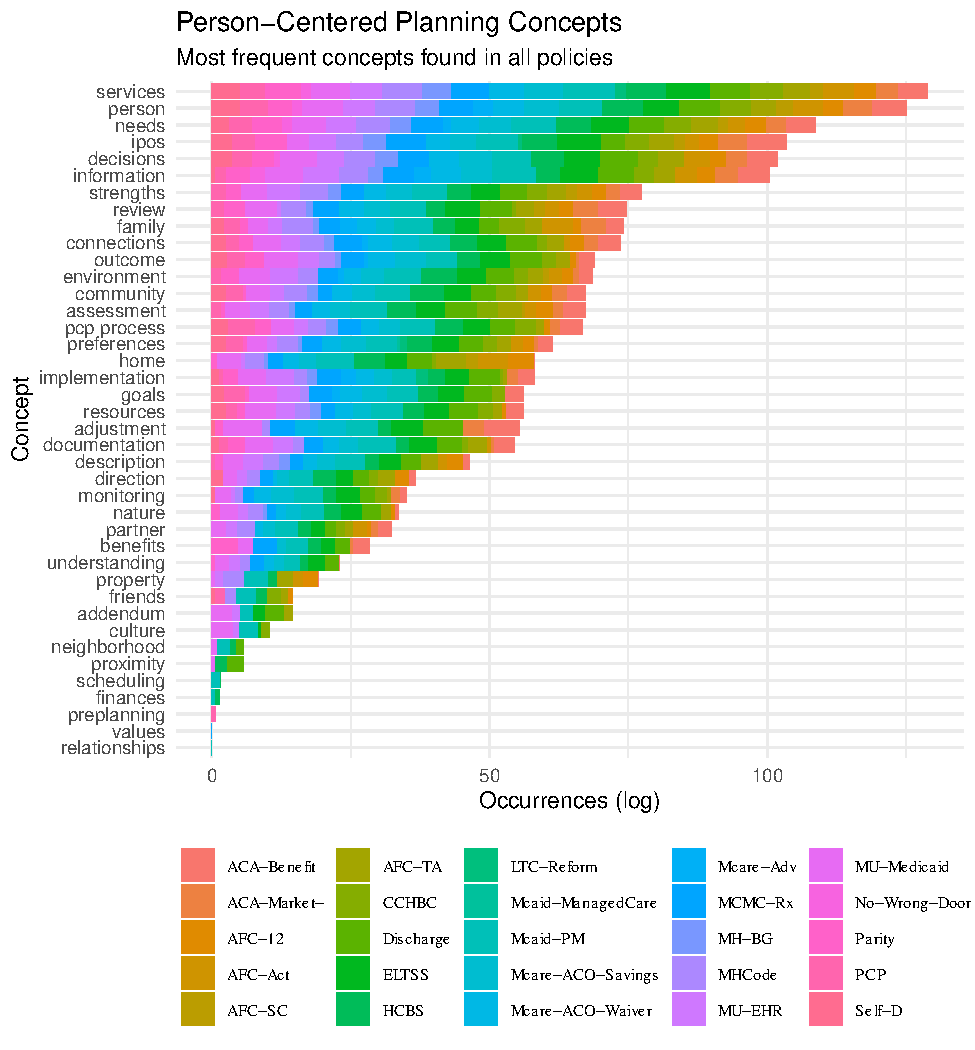
\includegraphics{person_centered_files/figure-latex/plot_policy_concept-1.pdf}

An example may be helpful in understanding what goes into the chart above. For instance, the concept of \emph{assessment} shown in the chart above occurs 1835 times across 22 separate policy documents.\footnote{The specific policies including this concept are: ACA-Benefit, ACA-Market-, AFC-12, AFC-Act, AFC-SC, AFC-TA, CCHBC, Discharge, ELTSS, HCBS, Mcaid-PM, Mcare-ACO-Savings, Mcare-ACO-Waiver, Mcare-Adv, MCMC-Rx, MH-BG, MHCode, MU-EHR, MU-Medicaid, No-Wrong-Door, Parity, PCP}

The table below shows a sample of the text from some of the policies where this concept is flagged:

\begin{tabular}{l|l|r}
\hline
doc\_id & text & sid\\
\hline
AFC-TA & Resident admission criteria ; resident assessment plan ; emergency admission ; resident care agreement ; physician 's instructions ; health care appraisal ( //) R. Resident admission and discharge policy ; house rules ; emergency discharge ; change of residency ; restricting resident 's ability to make living // STATE OF MICHIGAN Department of Licensing and Regulatory Affairs of ADULT FOSTER CARE GROUP HOME TECHNICAL ASSISTANCE MANUAL arrangements prohibited ; provision of resident records at time of discharge ( //) R. Resident care ; licensee responsibilities ( / / ) . & 11\\
\hline
AFC-TA & ( d ) " Assessment plan " means a written statement which is prepared in cooperation with a responsible agency or person and which identifies the specific care and maintenance , services , and resident activities appropriate for each individual resident 's physical and behavioral needs and wellbeing and the methods of providing the care and services , taking into account the preferences and competency of the individual . & 55\\
\hline
AFC-TA & Assist with the completion of a written assessment plan at the time of admission and review with the licensee at least annually . & 71\\
\hline
AFC-TA & [ ] ( j ) " Health care appraisal " means a licensed physician 's , licensed physician 's assistant 's , or registered nurse 's statement that provides an assessment of the general physical condition of a resident . & 114\\
\hline
AFC-TA & // STATE OF MICHIGAN Department of Licensing and Regulatory Affairs of ADULT FOSTER CARE GROUP HOME TECHNICAL ASSISTANCE MANUAL ( i ) Assessment planning and the establishment of an IPOS . & 173\\
\hline
AFC-TA & ( c ) Be capable of assuring program planning , development , and implementation of services to residents consistent with the home 's program statement and in accordance with the resident 's assessment plan and care agreement . () & 369\\
\hline
AFC-TA & The consultant is to determine that the licensee has a training methodology in place that assures that all direct care staff are competent in providing the personal care , supervision and protection as identified in the facility 's program statement and admission / discharge policy as well as the individual assessment plans , health care appraisals and resident care agreements . & 445\\
\hline
AFC-TA & This can be accomplished by TB testing , x - ray , screening , an assessment or physical exam completed by the person 's physician or local health authority . & 471\\
\hline
AFC-TA & The home health aide can not be counted when determining the adequacy of on duty direct care staff that are required in the home in order to provide the services specified by the home 's resident assessments and resident care agreements or in determining the minimally required resident to staff ratio . () & 488\\
\hline
AFC-TA & A licensee shall have sufficient direct care staff on duty at all times for the supervision , personal care , and protection of residents and to provide the services specified in the resident 's resident care agreement and assessment plan . & 489\\
\hline
AFC-TA & For purposes of this rule " Sufficient direct care staff " is defined to mean the number of staff necessary to implement the care needs as indicated in the resident 's assessment plan , health care appraisal , and resident care agreement . & 491\\
\hline
AFC-TA & Resident assessment plans g . & 499\\
\hline
AFC-TA & Resident admission criteria ; resident assessment plan ; emergency admission ; resident care agreement ; physician 's instructions ; health care appraisal . & 641\\
\hline
AFC-TA & // STATE OF MICHIGAN Department of Licensing and Regulatory Affairs of ADULT FOSTER CARE GROUP HOME TECHNICAL ASSISTANCE MANUAL Technical Assistance Continuous nursing care is defined as requiring a nurse 's presence to provide ongoing nursing assessments , judgments and / or interventions . & 645\\
\hline
AFC-TA & A licensee shall not accept or retain a resident for care unless and until the licensee has completed a written assessment of the resident and determined that the resident is suitable pursuant to all of the following provisions : Technical Assistance & 648\\
\hline
HCBS & This commenter urged CMS to ensure that individuals have assessments of need to ensure they are not placed in the wrong settings . & 293\\
\hline
HCBS & Sections ( c ) , ( i ) and ( k ) of the Act all require that individuals have an individual assessment of needs that includes the individual 's needs , strengths , preferences and goals for servicesupport provided under the respective authorities . & 294\\
\hline
HCBS & While we understand that there may be circumstances in which an individual 's needs require a different level of service , we expect that the assessment of functional need , the person - centered plan and the availability of HCBS will be able to address an individual 's changing needs . & 378\\
\hline
HCBS & One commenter supports the regulation , but believes the rule should go further and require living units to have access to food storage and preparation space ( with the caveat that stoves or microwaves could be removed if the assessment documented that it would be a danger because of the resident 's cognitive impairment ) . & 529\\
\hline
HCBS & This review will also include assessment of how the settings allow for full integration into the broader community . & 663\\
\hline
HCBS & States are responsible for determining the provider qualifications of the entities who will conduct the assessments and PCP process as long as the requirements in the final regulations have been met . & 968\\
\hline
HCBS & The regulation already specifies the involvement of an individual 's representative in the evaluation of eligibility ( . ) , independent assessment ( . ) , and person - centered service plan ( . ) . & 996\\
\hline
HCBS & Several commenters asked how frequently the assessment must be made if the condition causing the modification of the " additional conditions " was not likely to improve . & 1020\\
\hline
HCBS & We also state in the rule that reviews and any needed revision of the independent assessment and the person - centered service plan , must occur at least every months , when the individual 's circumstances or needs change significantly , and at the request of the individual . & 1023\\
\hline
HCBS & While ( i ) ( ) ( F ) ( i ) requires that the independent assessment include an objective evaluation of an individual 's inability or need for assistance to perform or more ADLs , this is only a suggested element at ( i ) ( ) ( D ) ( i ) and thus , not required for an individual to be determined eligible for ( i ) State plan HCBS . & 1165\\
\hline
HCBS & This suggestion is already captured in . ( a ) ( ) where the regulation requires the assessment to " ... include the opportunity for the individual to identify other persons to be consulted , such as , but not limited to , the individual 's spouse , family , A couple of commenters stressed the importance that FFP be available for evaluations even when an individual is subsequently found ineligible for section ( i ) of the Act services . & 1169\\
\hline
HCBS & As stated in section III.N .. of the preamble to the proposed rule , FFP is available for evaluation and assessment as administration of the approved state plan prior to an individual 's determination of eligibility for and receipt of other section ( i ) of the Act services . & 1170\\
\hline
HCBS & If the individual is found not eligible for the State plan HCBS benefit , the state may claim the evaluation and assessment as administration , even though the individual would not be considered to have participated in the benefit for purposes of determining the annual number of individuals served by the benefit . & 1171\\
\hline
HCBS & Some commenters requested clarification regarding level of need , as defined by the state and provider , including whether a state may leverage existing and / or specific instruments that are used to determine HCBS waiver eligibility in order to determine whether a beneficiary meets the State plan HCBS needs assessment criteria for participation , understanding that the State plan HCBS benefit eligibility criteria must be less stringent than that used for HCBS waiver programs . & 1172\\
\hline
HCBS & One commenter indicated that if states establish needs - based criteria for each specific service that an individual receives , it would add to the complexity of the assessment service planning , the overall costs of program administration , and potential beneficiary and family caregiver confusion . & 1175\\
\hline
MHCode & () " Incapacitated " means that an individual , as a result of the use of alcohol or other drugs , is unconscious or has his or her mental or physical functioning so impaired that he or she either poses an immediate and substantial danger to his or her own health and safety or is endangering the health and safety of the public . () " IPOS " or " plan of services " means a written IPOS developed with a recipient as required by section . () " Intellectual disability " means a condition manifesting before the age of years that is characterized by significantly subaverage intellectual functioning and related limitations in or more adaptive skills and that is diagnosed based on the following assumptions : ( a ) Valid assessment considers cultural and linguistic diversity , as well as differences in communication and behavioral factors . & 107\\
\hline
MHCode & ( d ) Submit to the members of the house and senate standing committees and appropriation subcommittees with legislative oversight of mental health matters an annual report summarizing its assessment of the mental health needs of the state and incorporating information received from CMH service s programs under section . & 286\\
\hline
MHCode & The record shall contain at a minimum a written assessment and IPOS for the patient , a statement of the purpose of hospitalization or treatment , a description of any tests and examinations performed , and a description of any observations made and treatments provided . & 569\\
\hline
MHCode & ( c ) Sample assessments of families receiving family support subsidy payments including adequacy of subsidy and need for services not available . & 792\\
\hline
MHCode & The office shall do all of the following : ( a ) Assess the mental health needs of multicultural populations in the state . & 828\\
\hline
MHCode & ( b ) Identification , assessment , and diagnosis to determine the specific needs of the recipient and to develop an IPOS . & 1018\\
\hline
MHCode & ( h ) Screening and assessment procedures . & 1055\\
\hline
MHCode & Sec . () The board of a CMH services program shall do all of the following : ( a ) Annually conduct a needs assessment to determine the mental health needs of the residents of the county or counties it represents and identify public and nonpublic services necessary to meet those needs . & 1218\\
\hline
MHCode & It is the responsibility of the CMH services program to involve the public and private providers of mental health services located in the county or counties served by the CMH program in this assessment and service identification process . & 1220\\
\hline
MHCode & The needs assessment shall include information gathered from all appropriate sources , including CMH waiting list data and school districts providing special education services . & 1221\\
\hline
MHCode & ( b ) Annually review and submit to the department a needs assessment report , annual plan , and request for new funds for the CMH services program . & 1222\\
\hline
MHCode & The standard format and documentation of the needs assessment , annual plan , and request for new funds shall be specified by the department . & 1223\\
\hline
MHCode & ( c ) In the case of a county CMH agency , obtain approval of its needs assessment , annual plan and budget , and request for new funds from the board of commissioners of each participating county before submission of the plan to the department . & 1224\\
\hline
MHCode & In the case of a CMH organization , provide a copy of its needs assessment , annual plan , request for new funds , and any other document specified in accordance with the terms and conditions of the organization 's inter- local agreement to the board of commissioners of each county creating the organization . & 1225\\
\hline
MHCode & In the case of a CMH authority , provide a copy of its needs assessment , annual plan , and request for new funds to the board of commissioners of each county creating the authority . & 1226\\
\hline
\end{tabular}

\hypertarget{research}{%
\chapter{Informed by (and Informing) Research}\label{research}}

Some activities related to person-centered planning are addressed in existing research.\footnote{For instance, \emph{goals and planning}, \emph{feedback and monitoring}, and similar activities defined by the \href{https://www.humanbehaviourchange.org/resources/behavioural-science/25/description}{Behaviour Change Intervention Ontology (BCIO)} have related research available.} In these instances, our goal would be to connect-the-dots between research and practice by making this knowledge available. In order to remain aligned with national efforts\footnote{NQF's \href{http://www.qualityforum.org/WorkArea/linkit.aspx?LinkIdentifier=id\&ItemID=91382}{Person-Centered Planning and Practice Project}, references `\emph{a research agenda to advance and promote person-centered planning in LTSS}'} in this area, initial steps would include:

\begin{itemize}
\tightlist
\item
  mapping of person-centered planning concepts to researched interventions
\item
  literature review and meta-analyses of PCP-related practices, to build a base of best practices and evidence for effectiveness
\item
  identification of gaps in existing research knowledge related to PCP
\end{itemize}

\hypertarget{curriculum}{%
\chapter{Shared Training Curriculum}\label{curriculum}}

To translate this information into action, various audiences need to be trained in person-centered practice, using the foundational concepts identified and defined above. Work in developing these trainings includes:

\begin{itemize}
\tightlist
\item
  Identification of key audiences
\item
  Evaluation of potential training modalities based on key features
\item
  Developing a standard base curriculum as well as specialty topics for specific audiences
\end{itemize}

\hypertarget{measure}{%
\chapter{Person-Centered Measurement Framework}\label{measure}}

If the entire system of services and supports is intended to be person-centered, its performance should be measured within a framework that also person-centered. Many existing quality measures and data collection systems were not developed with this in mind. Thus, it will be important to develop a larger framework within which existing measures can be situated. This allows the system to retain the quality measurement work that has been completed, while filling gaps that may lead to inconsistency and poor quality.

The measurement framework outlined here attempts to align with and fulfill the promise of current definitions of person-centered planning, as well as with existing and evolving standards in the fields of behavioral health and developmental disability services. Far from contradicting these standards, it attempts to provide a broader, person-centered context for the development of the system as a whole.

Ongoing work in this area would include:

\begin{itemize}
\tightlist
\item
  Developing a person-centered measurement framework
\item
  Conducting an inventory of available data assets at a state wide level
\item
  Classifying existing measurement and data collection efforts (e.g.~HEDIS, BH-TEDS, etc.) within the context of this framework
\item
  Gap analysis of current datasets and development of a plan to address measurement gaps.
\end{itemize}

\hypertarget{qol_def}{%
\section{What do we mean by `a better life'?}\label{qol_def}}

People have been asking themselves what it means to live a good life for thousands of years,\footnote{The philosopher Aristotle defined the highest good of human life as happiness, or flourishing (\emph{eudaimonia}). cf.~\emph{Nicomachean Ethics}} and it is among the most crucial questions for each of us to answer. For the purpose of this measurement framework, we will refer to the characteristics that make up a good life as \emph{quality of life}, or QOL for short, relying primarily on contemporary research to arrive at a common and usable definition.

\hypertarget{what-makes-a-good-definition}{%
\subsection{What makes a good definition?}\label{what-makes-a-good-definition}}

If we are going to try to define quality of life, it is important that our definition gets a few things right:\footnote{These considerations are drawn from \href{https://www.ncbi.nlm.nih.gov/pubmed/16162114}{Cummins, R. (2005). Moving from the quality of life concept to a theory. JIDR, 49(10), 699-706}.}

\begin{enumerate}
\def\labelenumi{\arabic{enumi}.}
\tightlist
\item
  \emph{Multiple dimensions}. A good life can only be described using multiple dimensions. These are influenced by personal factors, environmental factors, and the interaction between those factors.
\item
  \emph{Broad enough for everyone}. We should each want to apply the definition to our own lives. The basic characteristics of a good life are the same for all people, regardless of culture, gender, disability, etc.
\item
  \emph{Both subjective and objective}. People have different priorities. While a definition can point to objective facts related to QoL, it must include the point-of-view of the person who is living their life from day to day. Each dimension of a QoL model may have both objectively and subjectively defined indicators.
\end{enumerate}

Taken together, the criteria listed above seek to balance the abstract with the specific and to arrive at a definition which is well-rounded while also being understandable.

\hypertarget{what-makes-a-better-life}{%
\subsection{What makes a better life?}\label{what-makes-a-better-life}}

Keeping our key requirements in mind, we can draw from the broad reservoir of studies on QoL to find frameworks which are multi-dimensional\footnote{See systematic review of HRQoL recommending addition of individual and environmental characteristics: \href{https://www.ncbi.nlm.nih.gov/pmc/articles/PMC3548743/}{Bakas, T., et al.~(2012)}.}, cross-culturally relevant,\footnote{See \href{https://www.researchgate.net/profile/Mian_Wang4/publication/7801771_Cross-Cultural_Study_of_Quality_of_Life_Indicators/links/0deec52df448eac34d000000/Cross-Cultural-Study-of-Quality-of-Life-Indicators.pdf}{Schalock, R., et al.~(2005).}.} and which provide both subjective and objective indicators.

Below is a potential model listing essential dimensions of QoL:

\begin{table}

\caption{\label{tab:unnamed-chunk-13}QoL Dimensions}
\centering
\begin{tabular}[t]{l|l|l}
\hline
Area & Dimension & Example Indicators\\
\hline
Independence & Personal development & Education status, personal skills, ADLs, IADLs\\
\hline
 & Self-determination & Choices, autonomy, personal control, goals\\
\hline
Social participation & Interpersonal relations & Social networks, activities, relationships\\
\hline
 & Social inclusion & Community integration, participation, roles\\
\hline
 & Rights & Human (respect/dignity, equality), Legal\\
\hline
Well-being & Emotional well-being & Safety, positive experiences, self-concept, stress\\
\hline
 & Physical well-being & Health, nutrition, recreation/physical exertion\\
\hline
 & Material well-being & Financial status, employment, housing, possessions\\
\hline
\end{tabular}
\end{table}

Please note that the framework listed above is one of many potential models, each of which contains many of the same basic dimensions, and many were developed with populations having specific conditions. Some other broad-based models for review include:

\begin{itemize}
\tightlist
\item
  The \href{https://apps.who.int/iris/bitstream/handle/10665/77932/WHO_HIS_HSI_Rev.2012.03_eng.pdf?sequence=1\&isAllowed=y}{World Health Organization Quality of Life (WHOQOL)} domains.
\item
  The \href{https://ec.europa.eu/eurostat/statistics-explained/index.php?title=Quality_of_life_indicators}{Eurostat QoL indicators} show an example of QoL domains applied for entire countries alongside financial indicators such as gross domestic product (GDP).
\item
  Healthy People 2020 has selected a subset of measures for monitoring health-related QoL and well-being in the United States. See their \href{https://www.healthypeople.gov/sites/default/files/HRQoLWBFullReport.pdf}{Foundation Health Measure Report: Health-Related QoL and Well-Being}.
\end{itemize}

\hypertarget{benefits-of-a-qol-perspective}{%
\section{Benefits of a QoL Perspective}\label{benefits-of-a-qol-perspective}}

\hypertarget{what-other-frameworks-exist}{%
\subsection{What other frameworks exist?}\label{what-other-frameworks-exist}}

One might well ask: \emph{Is quality of life the only potential framework that we could use to measure improvement?} The answer is \emph{No}, so it is worth discussing other options and briefly reviewing the attributes of each. Other options include:

\begin{itemize}
\tightlist
\item
  \emph{Symptom reduction}: Measurement of reduction in symptoms related to specific diagnosable conditions. Symptom scales such as the \href{https://www.phqscreeners.com/sites/g/files/g10049256/f/201412/PHQ-9_English.pdf}{PHQ-9}, \href{}{GAD-7} and other tools have commonly been used to measure the impact of treatments on specific conditions, but they are more challenging to use for people with multiple co-occuring conditions (MCC).
\item
  \emph{Improving functional status}: Most currently used assessment tools address functional status, measuring the impact of various conditions on broader life areas in terms of their impact on functional ability. These are broader than symptom scales, and can detect the impact of various symptoms on a particular functional domain.
\item
  \emph{Health-related quality of life (HRQoL)}: HRQoL addresses a subset of QoL domains which are related to perceived physical and mental health. These models typically exclude non-medical areas such as education or rights, focusing on physical domains like `mobility'.
\end{itemize}

\hypertarget{why-is-a-quality-of-life-framework-better-than-others}{%
\subsection{Why is a quality of life framework better than others?}\label{why-is-a-quality-of-life-framework-better-than-others}}

A QoL approach has the following benefits over the approaches mentioned above:

\textbf{Strengths-based}: A QoL approach asks people what they want their lives to be and encourages them to work toward that vision. Rather than focusing on needs or deficits, it aspires to use a person's strengths to improve his or her life.\footnote{See the MDHHS PCP Policy value that ``The PCP approach identifies the person's strengths, goals, choices\ldots{} and desired outcomes.'' (p.~4)}

\textbf{Inclusive}: Instruments and measures from each of the other areas can be used as a part of the QoL framework, since it is broad enough to include each of these areas, and they each contribute to it. A QoL approach does not neglect the value of functional gains or symptom reduction, but values these as contributors to overall quality of life. For instance, if a person experiences an alleviation of their depressive symptoms using the PHQ-9, this would be seen as contributing toward the individual's QoL in the area of `Emotional Well-being'.

\textbf{Contextual}: An approach which focuses on only a portion of an individual's life, such as mobility or anxiety symptoms, is likely to miss out on the bigger picture. It may also inadvertently create siloes among the individuals supporting the person. For instance, more recent evaluations have criticized the HRQoL approach as failing to ``sufficient emphasis on mental and social domains\ldots that are essential to people.''\footnote{Read \href{https://www.ncbi.nlm.nih.gov/pmc/articles/PMC4031380/}{Pietersma, S., et al.~(2013)} regarding domains of quality of life.} The broader focus on QoL which is proposed here is aligned with our evolving understanding of several areas, each of which stresses the critical relationship between each of us and our communities and surroundings:

\begin{itemize}
\tightlist
\item
  \emph{Social Determinants of Health} (SDoH): A vast and growing body of \href{https://www.cdc.gov/socialdeterminants/research/index.htm}{research} indicates that the places and conditions in which we live are intrinsically tied to the quality of our lives and the likelihood of achieving positive outcomes from the supports and services we receive.
\item
  \emph{Trauma-Informed Care}: More and more models for service provision, informed by research and by the lived experience of trauma survivors, are founded on the recognition that adverse events in our relationships and in our lived environment can have a profound and lifelong impact on our lives.\footnote{For a recent review of these models, see: \href{https://www.ncbi.nlm.nih.gov/pubmed/30079827}{Purtle, J. (2018). Trauma, Violence, \& Abuse}.}
\item
  \emph{Supports Paradigm}: A model, prevalent in the IDD supports system, that views a person's functioning as the match between their individual capacity and the environment in which they are expected to live and work.\footnote{See \href{https://www.ncbi.nlm.nih.gov/pubmed/19368481}{Thompson, et al.~(2009)} on conceptualizing support needs.} In this model, supports are viewed as a way to supplement the persons strengths and to help match those to the person's environment.
\end{itemize}

\hypertarget{appendix}{%
\chapter{Appendix}\label{appendix}}

\hypertarget{alignment-with-of-measures-with-existing-requirements}{%
\section{Alignment with of Measures with Existing Requirements}\label{alignment-with-of-measures-with-existing-requirements}}

\hypertarget{alignment-with-federal-medicaid-requirements}{%
\subsection{Alignment with Federal Medicaid Requirements}\label{alignment-with-federal-medicaid-requirements}}

\hypertarget{alignment-with-provider-requirements}{%
\subsection{Alignment with Provider Requirements}\label{alignment-with-provider-requirements}}

\emph{Feasible for Implementation}: Multiple pragmatic trials have demonstrated that the use of symptom scales are both feasible to implement on a large scale\footnote{See the large scale implementations cited in \href{https://ps.psychiatryonline.org/doi/full/10.1176/appi.ps.201500439\#T1}{Fortney, J. C., et al.~(2016). A tipping point for measurement-based care. Psychiatric Services, 68(2), 179-188.}.} and acceptable to people receiving services.\footnote{\href{https://www.bmj.com/content/338/bmj.b663.long}{Dowrick, C., et al.~(2009)} report that the use of instruments increase confidence in providers' accuracy and management.}

\emph{Provider Accreditation}: New standards for Joint Commission accreditation (effective 2018)\footnote{See Joint Commission \href{https://www.jointcommission.org/assets/1/6/Approved_BHC_outcome_meas_2018.pdf}{\emph{Standard CTS.03.01.09}, sections \emph{EP1-3}}.} require that an organization (a) ``uses a standardized tool or instrument to monitor individuals progress in achieving\ldots{} goals'', (b) ``gathers and analyzes data generated through standardized monitoring, and results used to inform goals and objectives of individual's plan'', and (c) ``evaluates outcomes of\ldots{} services\ldots{} by aggregating and analyzing data collected through the standardized monitoring effort.''

\emph{Diagnostic Practice}: The most recent diagnostic manual (DSM-5) includes \href{https://www.psychiatry.org/psychiatrists/practice/dsm/educational-resources/assessment-measures}{assessment measures} which were ``developed to be administered at the initial patient interview and to monitor treatment progress.''

\hypertarget{framework-for-measurement}{%
\section{Framework for Measurement}\label{framework-for-measurement}}

\hypertarget{scope}{%
\subsection{Scope}\label{scope}}

\begin{figure}
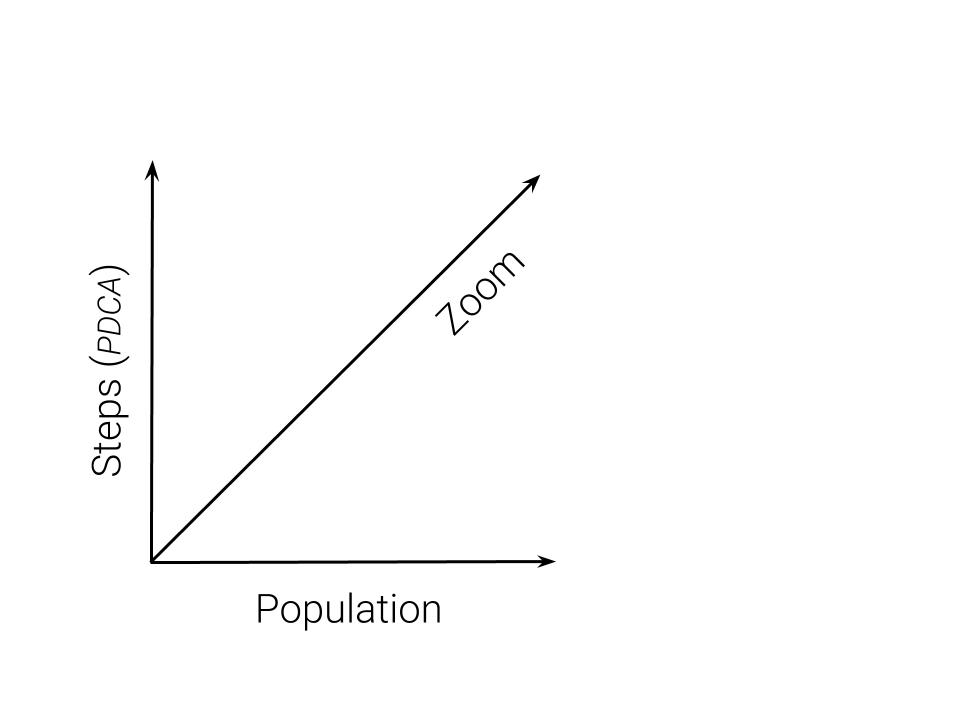
\includegraphics[width=24in]{_bookdown_files/img/QoL Framework Scope} \caption{Scope of framework}\label{fig:unnamed-chunk-14}
\end{figure}

A conceptual framework as comprehensive as the one we are proposing runs the risk of becoming overwhelmingly complex and unwieldy to implement. So, before diving into any details, we want to begin by sketching out a simple way to think about the scope of the framework required to systematically measure person-centered planning and its impact of quality of life. Having a definition of scope can help us answer questions such as:

\begin{itemize}
\tightlist
\item
  What types of data are included, and what types of measures?\\
\item
  How will we know when the framework is fully implemented?\\
\item
  Does this fit with other work that we are doing?
\end{itemize}

We can define the scope of the framework using three-dimensions (\emph{\protect\hyperlink{zoom}{depth}, \protect\hyperlink{pop}{breadth}, and \protect\hyperlink{steps}{height}}) as defined below:

\textbf{Depth} (a.k.a. \emph{Zoom}): Does the framework allow for understanding at various levels of `resolution', from the most immediate (i.e.~\emph{the individual person}) to the aggregate (i.e.~\emph{the population}) and other levels inbetween (e.g.~\emph{the organization, team, etc.})?

\textbf{Breadth} (a.k.a. \emph{Population}): Can the framework apply to all people who are planning to improve their lives with the help of services and supports?\footnote{I.e., to all `populations' around which systems have been developed (\emph{SMI, SED, IDD, SUD, etc.}). Since different data exists for each group, evaluating alignment is key.}

\textbf{Height} (a.k.a. \emph{Steps}): Does the framework allow for understanding of each of the steps in the \protect\hyperlink{pcpdca}{person-centered PDCA process} discussed above?

\begin{figure}
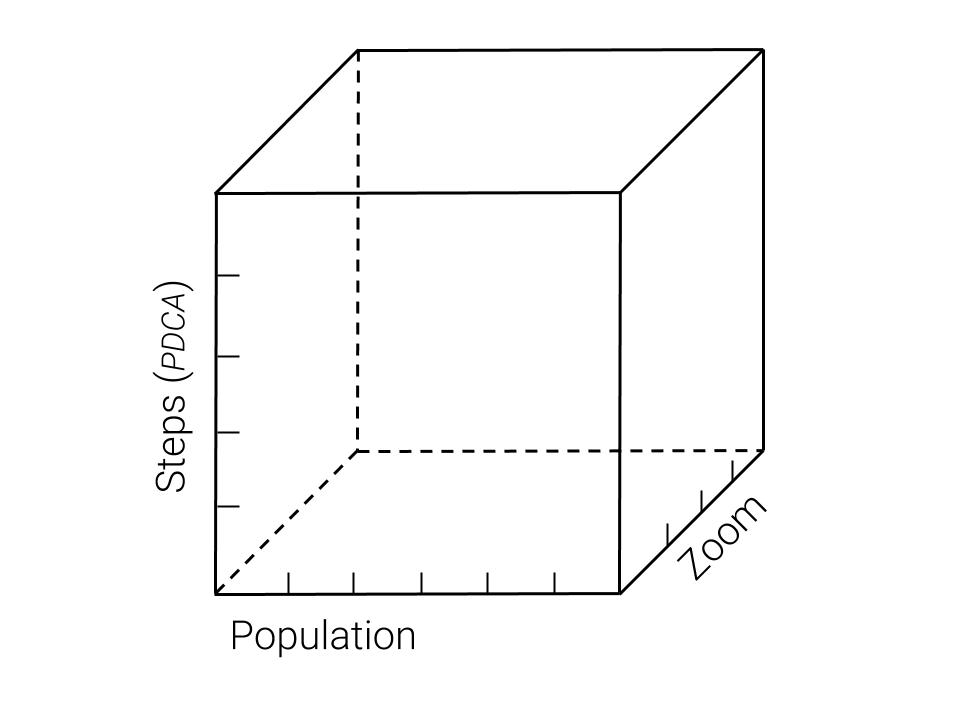
\includegraphics[width=24in]{_bookdown_files/img/QoL Framework Cube} \caption{If it was a cube...}\label{fig:unnamed-chunk-15}
\end{figure}

If we think about the framework as a cube made of these three dimensions, then developing the measurement framework can begin by making certain that data is collected:

\begin{itemize}
\tightlist
\item
  at each step of the person-centered PDCA process (\emph{height})
\item
  for people across all populations (\emph{breadth})
\item
  which can be aggregated at various levels of the system (\emph{depth})
\end{itemize}

So, speaking \emph{very} broadly, if our cube has data elements/measures at each intersection of the three dimensions, then it allows for at least a basic understanding of people's needs, planning, and services as these contribute to improved lives. In reality, there will always be additional data that can be collected and novel ways of combining that data, just as there continue to be additional books and songs written describing the human experience.

The next sections define each of the dimensions listed above, and how they relate to one another, in greater detail. Based on these details, it will be possible to begin a practical gap analysis to assess how closely the system's current data assets match the scope of the framework. Please note that this paper does not develop or identify specific measures, except as illustrations of how individual data elements or metrics \emph{might} fit into the overall framework.

\hypertarget{steps}{%
\subsection{Steps}\label{steps}}

\hypertarget{plan}{%
\subsubsection{Plan}\label{plan}}

\textbf{Understand Quality of Life.}

\textbf{Understand Needs Related to QoL.} The table below identifies example variables from required assessments which relate to the QoL domains outlined above.\footnote{Assessments included are the \href{http://aaidd.org/sis}{\emph{Supports Intensity Scale (SIS)}}, the \href{http://www2.fasoutcomes.com/Content.aspx?ContentID=12}{\emph{Child and Adolescent Functional Assessment Scale (CAFAS)}}, the \href{https://cchealth.org/mentalhealth/pdf/LOCUS.pdf}{\emph{Level of Care Utilization System (LOCUS)}}, and the \href{http://gaincc.org/}{\emph{Global Appraisal of Individual Needs (GAIN)}}} While this is not an exhaustive mapping, it shows how the assessment of personal needs (\emph{from the ``Plan'' step of PDCA}) relate to quality of life domains across multiple populations.

\begin{table}

\caption{\label{tab:unnamed-chunk-16}Sample: Need Assessment and Related QoL Dimensions}
\centering
\begin{tabular}[t]{l|l|l|l|l}
\hline
Dimension & SIS Subscale & CAFAS Subscale & LOCUS Dimension & GAIN Item\\
\hline
Personal development & Health \& Safety & School/Work &  & \\
\hline
 & Protection/Advocacy & Thinking &  & \\
\hline
 & Behavioral Support &  &  & \\
\hline
Self-determination & Protection/Advocacy &  & Engagement & \\
\hline
Interpersonal relations & Social Activities & Home &  & \\
\hline
Social inclusion & Community Living & Community &  & Living Situation\\
\hline
 & Social Activities &  &  & Environment\\
\hline
Rights & Protection/Advocacy &  &  & Legal\\
\hline
 & Health \& Safety &  &  & \\
\hline
Emotional well-being & Behavioral Support & Moods/Emotions & Risk of Harm & Emotional health\\
\hline
 & Health \& Safety & Behavior &  & \\
\hline
Physical well-being & Medical Support & Self-Harm & Co-Morbidity & Physical health\\
\hline
 & Health \& Safety &  & Risk of Harm & Disease prevention\\
\hline
Material well-being & Employment & Material Needs &  & Vocational\\
\hline
\end{tabular}
\end{table}

As mentioned above, the table above is intended to illustrate how assessments of need can be tied to QoL domains, but is not comprehensive.\footnote{For the SIS instrument, this table relied on the mapping described in \href{https://biblio.ugent.be/publication/1169626/file/6748818.pdf}{Van Loon, J., et al.~(2010). \emph{Assessing individual support needs to enhance personal outcomes}. Exceptionality, 18(4), 193-202}.} The actual mapping will need to be done at the level of specific questions, as opposed to subscales which are not as likely to fit neatly within a single QoL domain. Note that instruments which contain a larger number of items (such as the SIS) are likely to have greater coverage of QoL domains than instruments with a smaller number of items (such as the LOCUS).

\hypertarget{do}{%
\subsubsection{Do}\label{do}}

\hypertarget{check}{%
\subsubsection{Check}\label{check}}

When are measures taken?

What types of measures relate to what parts of the PCP process?

\hypertarget{act}{%
\subsubsection{Act}\label{act}}

\hypertarget{pcp-based-episodes}{%
\subsubsection{PCP-based Episodes}\label{pcp-based-episodes}}

Improvement takes time, both in our personal lives and in our collective work as organizations and systems. Various frameworks have been developed to help evaluate improvement over time, many of which rely on the concept of ``episodes'': periods of time which characterized by specific events or attributes. For instance\ldots{}

\begin{itemize}
\tightlist
\item
  an admission to treatment is used to define an episode in the \emph{Substance Abuse and Mental Health Services Administration} (SAMHSA) \href{https://www.samhsa.gov/data/data-we-collect/teds-treatment-episode-data-set}{\emph{Treatment Episode Data Set} (TEDS)}
\item
  the course of a particular illness is used to define an episode in the \emph{National Quality Forum}'s \href{https://www.qualityforum.org/Publications/2010/01/Measurement_Framework__Evaluating_Efficiency_Across_Patient-Focused_Episodes_of_Care.aspx}{Patient-Focused Episodes of Care}
\end{itemize}

Neither of the approaches above is optimal for understanding the effectiveness of the implementation of a person-centered plan. The admission-based approach will create longer episodes for long-term services and supports which do not correspond to revisions of the person-centerd plan and the effect of those revisions on quality of life. The illness-based approach will be overly reductive for people with multiple, concurrent conditions, lifelong conditions, or whose social and environmental conditions have a strong adverse impact on their quality of life.

If the person-centered planning (and doing, checking, acting) process is to be the primary catalyst for improvement of life using Medicaid supports and services, then that process should be used to define episodes for improvement. The broader `episode' of the PCP process would correspond to the period of time during which the person is receiving services, while also marking the interval between the plan and its next subsequent revision. If person-centered planning is expected to be creative, collaborative, and dynamic, then different `visions and revisions' of the plan will be longer or shorter. For instance, if a person develops a plan but soon realizes that it is not helping them to achieve the life goals they intended to, then the plan would be revised and the PCP cycle would be relatively short.

\hypertarget{zoom}{%
\subsection{Zoom}\label{zoom}}

\hypertarget{pop}{%
\subsection{Population}\label{pop}}

  \bibliography{book.bib,packages.bib}

\end{document}
